\documentclass[portrait,final,a0paper,fontscale=0.277]{baposter}

\usepackage{calc}
\usepackage{graphicx}
\usepackage{amsmath}
\usepackage{amssymb}
\usepackage{relsize}
\usepackage{multirow}
\usepackage{rotating}
\usepackage{bm}
\usepackage{url}
\usepackage{graphicx}
\usepackage{multicol}
% \usepackage{subfigure}
\usepackage[export]{adjustbox}% http://ctan.org/pkg/adjustbox

%\usepackage{times}
%\usepackage{helvet}
%\usepackage{bookman}
\usepackage{palatino}

\newcommand{\captionfont}{\footnotesize}

\graphicspath{{images/}{../images/}}
\usetikzlibrary{calc}

%%%%%%%%%%%%%%%%%%%%%%%%%%%%%%%%%%%%%%%%%%%%%%%%%%%%%%%%%%%%%%%%%%%%%%%%%%%%%%%%
%%%% Some math symbols used in the text
%%%%%%%%%%%%%%%%%%%%%%%%%%%%%%%%%%%%%%%%%%%%%%%%%%%%%%%%%%%%%%%%%%%%%%%%%%%%%%%%

%%%%%%%%%%%%%%%%%%%%%%%%%%%%%%%%%%%%%%%%%%%%%%%%%%%%%%%%%%%%%%%%%%%%%%%%%%%%%%%%
% Multicol Settings
%%%%%%%%%%%%%%%%%%%%%%%%%%%%%%%%%%%%%%%%%%%%%%%%%%%%%%%%%%%%%%%%%%%%%%%%%%%%%%%%
\setlength{\columnsep}{1.5em}
\setlength{\columnseprule}{0mm}

%%%%%%%%%%%%%%%%%%%%%%%%%%%%%%%%%%%%%%%%%%%%%%%%%%%%%%%%%%%%%%%%%%%%%%%%%%%%%%%%
% Save space in lists. Use this after the opening of the list
%%%%%%%%%%%%%%%%%%%%%%%%%%%%%%%%%%%%%%%%%%%%%%%%%%%%%%%%%%%%%%%%%%%%%%%%%%%%%%%%
\newcommand{\compresslist}{%
\setlength{\itemsep}{1pt}%
\setlength{\parskip}{0pt}%
\setlength{\parsep}{0pt}%
}

%%%%%%%%%%%%%%%%%%%%%%%%%%%%%%%%%%%%%%%%%%%%%%%%%%%%%%%%%%%%%%%%%%%%%%%%%%%%%%
%%% Begin of Document
%%%%%%%%%%%%%%%%%%%%%%%%%%%%%%%%%%%%%%%%%%%%%%%%%%%%%%%%%%%%%%%%%%%%%%%%%%%%%%

\begin{document}

%%%%%%%%%%%%%%%%%%%%%%%%%%%%%%%%%%%%%%%%%%%%%%%%%%%%%%%%%%%%%%%%%%%%%%%%%%%%%%
%%% Here starts the poster
%%%---------------------------------------------------------------------------
%%% Format it to your taste with the options
%%%%%%%%%%%%%%%%%%%%%%%%%%%%%%%%%%%%%%%%%%%%%%%%%%%%%%%%%%%%%%%%%%%%%%%%%%%%%%
% Define some colors

%\definecolor{lightblue}{cmyk}{0.83,0.24,0,0.12}
\definecolor{lightblue}{rgb}{0.145,0.6666,1}

\hyphenation{resolution occlusions}
%%
\begin{poster}%
  % Poster Options
  {
  % Show grid to help with alignment
  grid=false,
  % Column spacing
  colspacing=1em,
  % Color style
  bgColorOne=white,
  bgColorTwo=white,
  borderColor=black,
  headerColorOne=red,
  headerColorTwo=red,
  headerFontColor=white,
  boxColorOne=white,
  boxColorTwo=lightblue,
  % Format of textbox
  textborder=roundedleft,
  % Format of text header
  eyecatcher=true,
  headerborder=closed,
  headerheight=0.135\textheight,
%  textfont=\sc, An example of changing the text font
  headershape=roundedright,
  headershade=shadelr,
  headerfont=\Large\bf\textsc, %Sans Serif
  textfont={\setlength{\parindent}{1.5em}},
  boxshade=plain,
%  background=shade-tb,
  background=plain,
  linewidth=2pt
  }
  % Eye Catcher
  {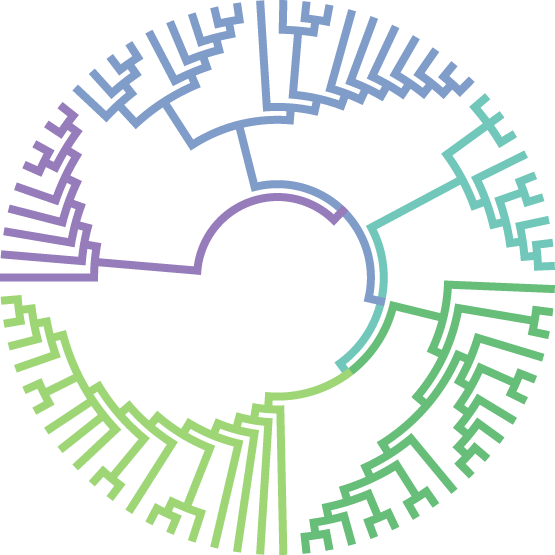
\includegraphics[height=7.0em]{images/rambaut_group_logo}} 
  % Title
  {\bf\textsc{Phylodynamics of Ebola in West Africa\linespread{0.25}\par}\vspace{0.25em}}
  % Authors
  {\textsc{Luiz Max de Carvalho$^{1,}$\footnote{{\small \texttt{lm.carvalho@ed.ac.uk} $^1$ Institute of Evolutionary Biology, University of Edinburgh, UK.}}\& Andrew Rambaut$^1$}\\
  }
  % University logo
  {
    
\includegraphics[height=7.0em]{images/edi_logo}
  }

%%%%%%%%%%%%%%%%%%%%%%%%%%%%%%%%%%%%%%%%%%%%%%%%%%%%%%%%%%%%%%%%%%%%%%%%%%%%%%
%%% Now define the boxes that make up the poster
%%%---------------------------------------------------------------------------
%%% Each box has a name and can be placed absolutely or relatively.
%%% The only inconvenience is that you can only specify a relative position 
%%% towards an already declared box. So if you have a box attached to the 
%%% bottom, one to the top and a third one which should be in between, you 
%%% have to specify the top and bottom boxes before you specify the middle 
%%% box.
%%%%%%%%%%%%%%%%%%%%%%%%%%%%%%%%%%%%%%%%%%%%%%%%%%%%%%%%%%%%%%%%%%%%%%%%%%%%%%
%     %
%     % A coloured circle useful as a bullet with an adjustably strong filling
%     \newcommand{\colouredcircle}{%
%       \tikz{\useasboundingbox (-0.2em,-0.32em) rectangle(0.2em,0.32em); \draw[draw=black,fill=lightblue,line width=0.03em] (0,0) circle(0.18em);}}

%%%%%%%%%%%%%%%%%%%%%%%%%%%%%%%%%%%%%%%%%%%%%%%%%%%%%%%%%%%%%%%%%%%%%%%%%%%%%%
  \headerbox{Motivation}{name=problem,column=0,row=0}{
%%%%%%%%%%%%%%%%%%%%%%%%%%%%%%%%%%%%%%%%%%%%%%%%%%%%%%%%%%%%%%%%%%%%%%%%%%%%%%
\begin{itemize}
 \item The 2013-2016 West African Ebola virus disease (EVD) epidemic was the largest in history;
 \item A massive international collaboration produced the most comprehensive data set for an acute virus to date (over 5\% sampling);
 \item Our challenge is to combine different sources of information (epidemiological, genetic, climatic, etc) to trace the epidemic and explain its mode and \texit{tempo}.
 \item Investigate the role of particular mutations in disease severity;
\end{itemize}
 }
%%%%%%%%%%%%%%%%%%%%%%%%%%%%%%%%%%%%%%%%%%%%%%%%%%%%%%%%%%%%%%%%%%%%%%%%%%%%%%
  \headerbox{Contributions}{name=contribution,column=0,below=problem}{
%%%%%%%%%%%%%%%%%%%%%%%%%%%%%%%%%%%%%%%%%%%%%%%%%%%%%%%%%%%%%%%%%%%%%%%%%%%%%%
Here I present my contributions to Dudas et al. (2016) and Diehl et al. (2016):
   \begin{itemize}
    \renewcommand{\labelitemi}{\tiny$\blacksquare$} 
    \item Generalised linear model (GLM) to study the association between a particular mutation, viral load and fatality rates;
    \item More GLMs, this time coupled with Stochastic Search Variable Selection (SSVS) to investigate the factors that drove the epidemic;
    \item Construction of (approximately) conditionally independent clusters combining incidence and phylogenetic data;
   \end{itemize}
}
%%%%%%%%%%%%%%%%%%%%%%%%%%%%%%%%%%%%%%%%%%%%%%%%%%%%%%%%%%%%%%%%%%%%%%%%%%%%%%
\headerbox{ Results }{name=results,column=1,span=2,row=0}{
\section*{ Did the GP-A82V mutation increase mortality?}
 \begin{tabular}{cc}
 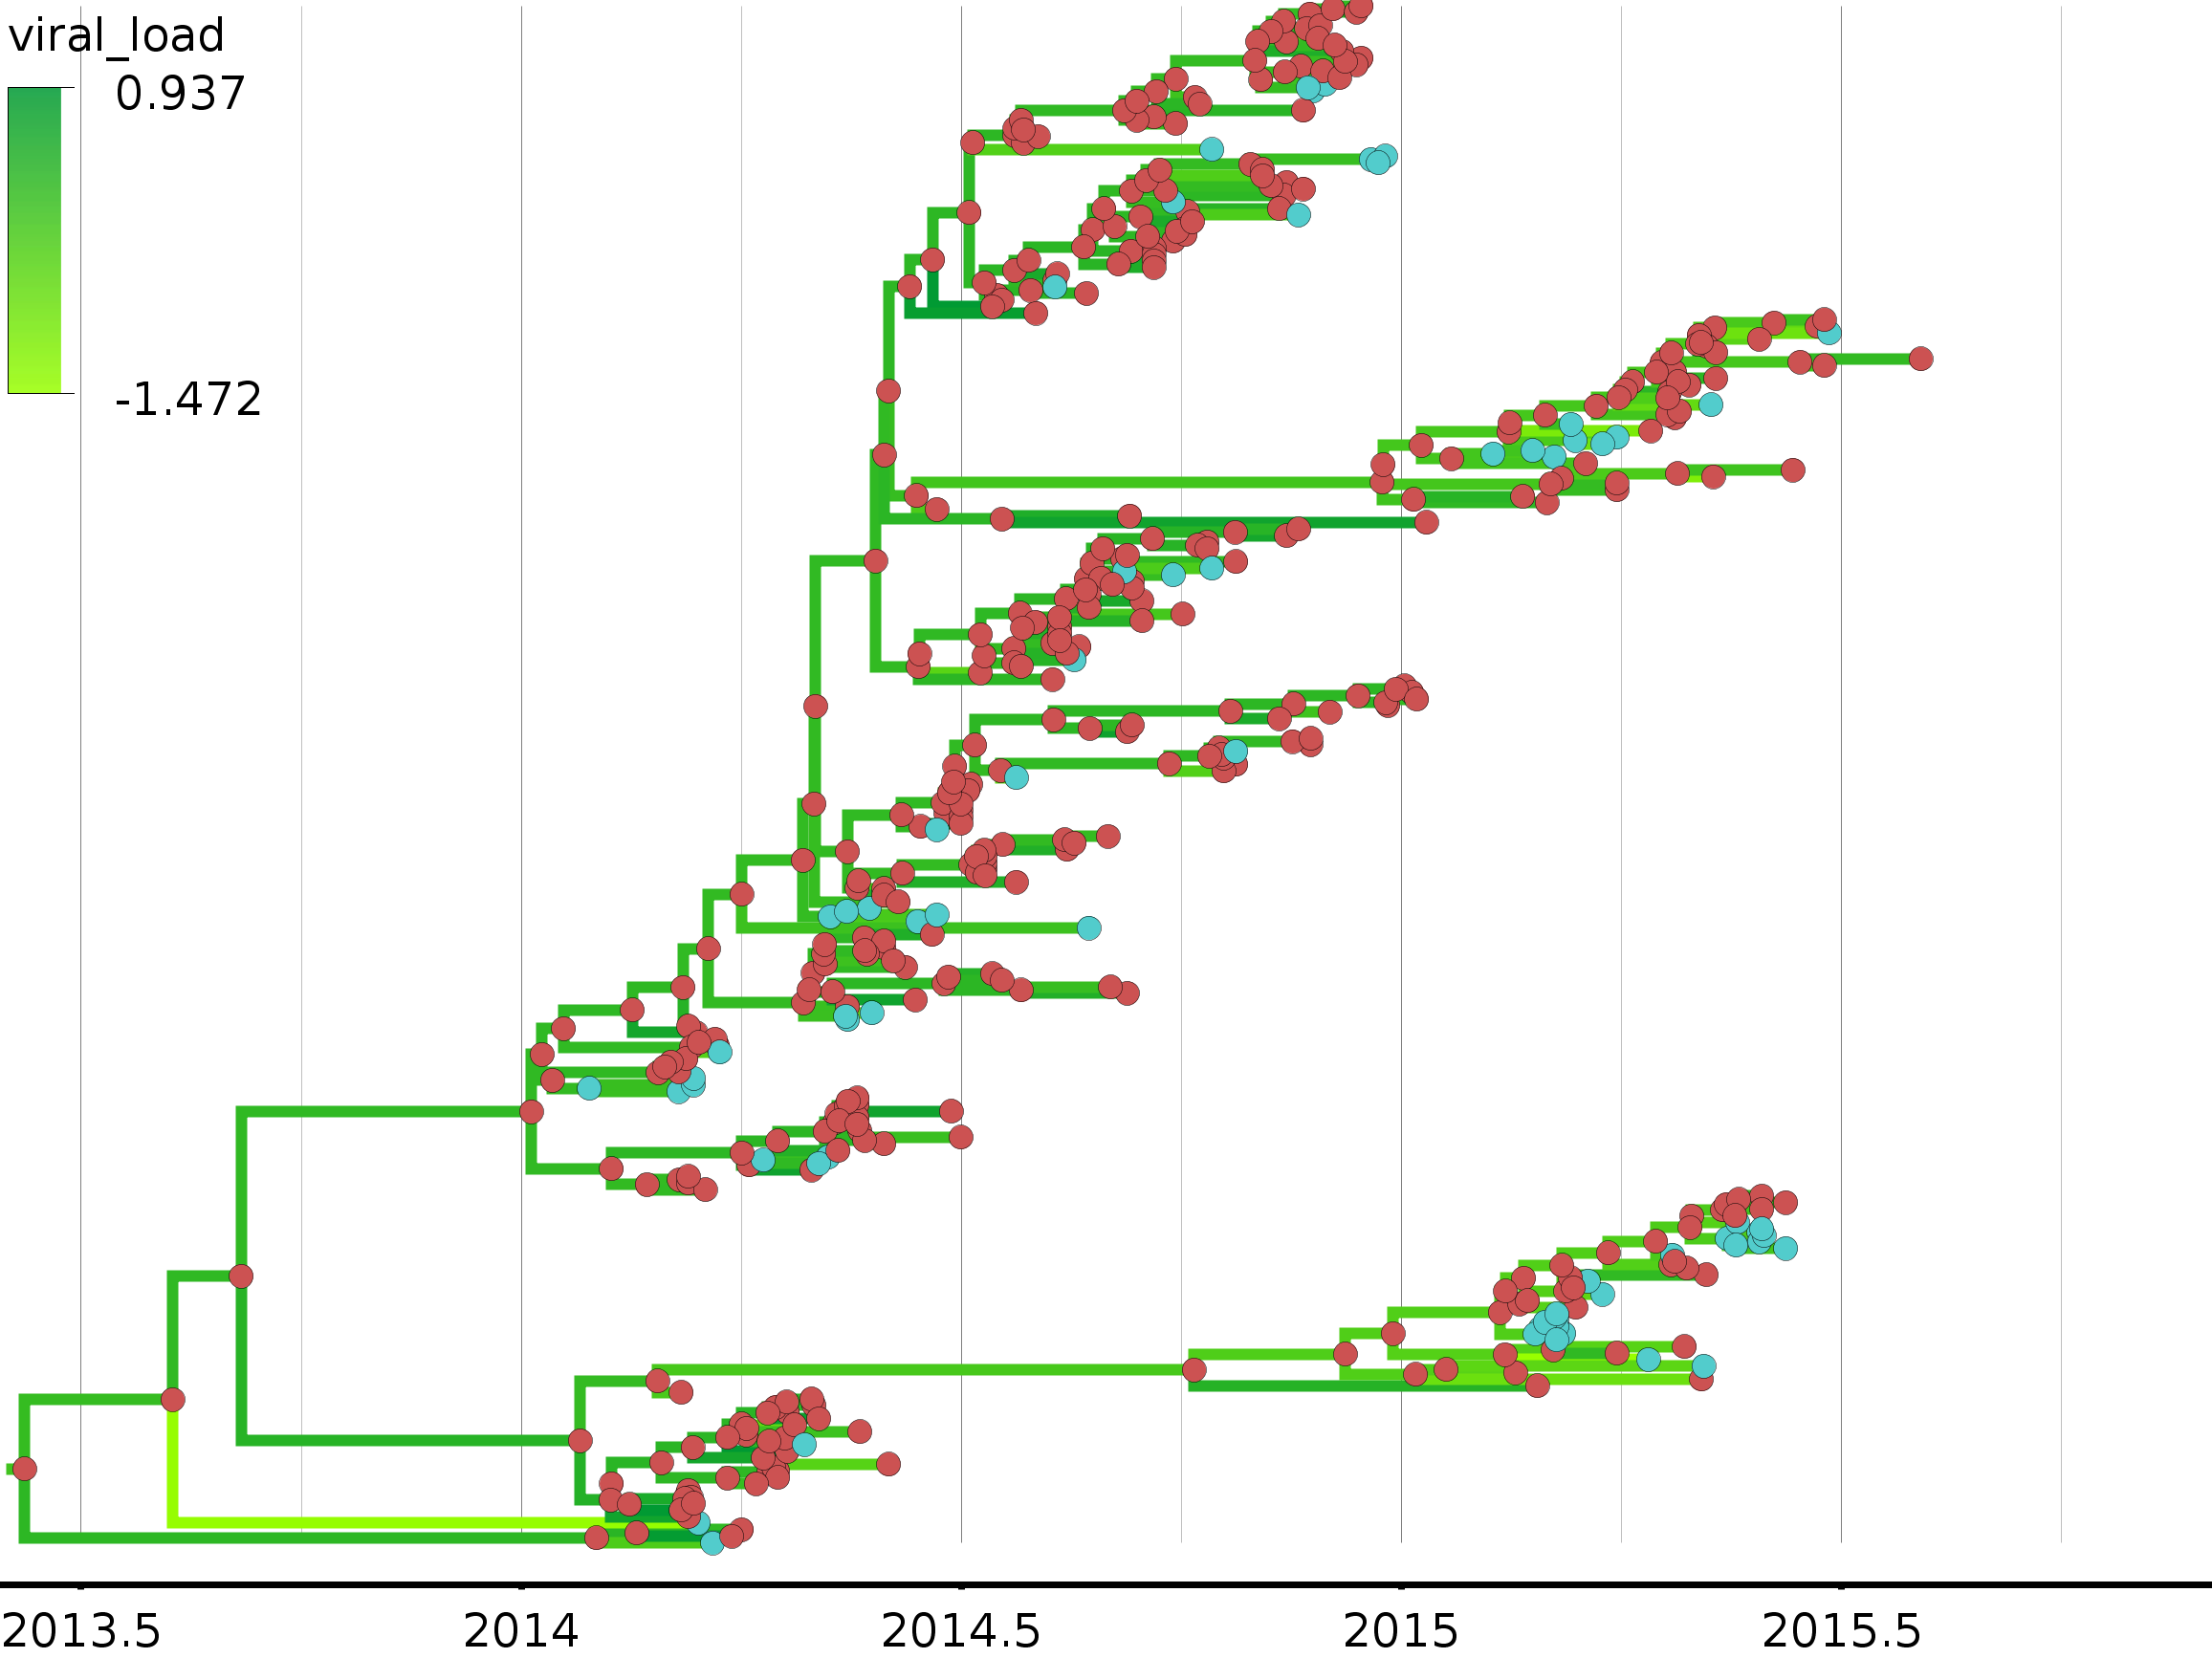
\includegraphics[scale=0.09,valign=c]{images/EVD_traits_tree.png} &
 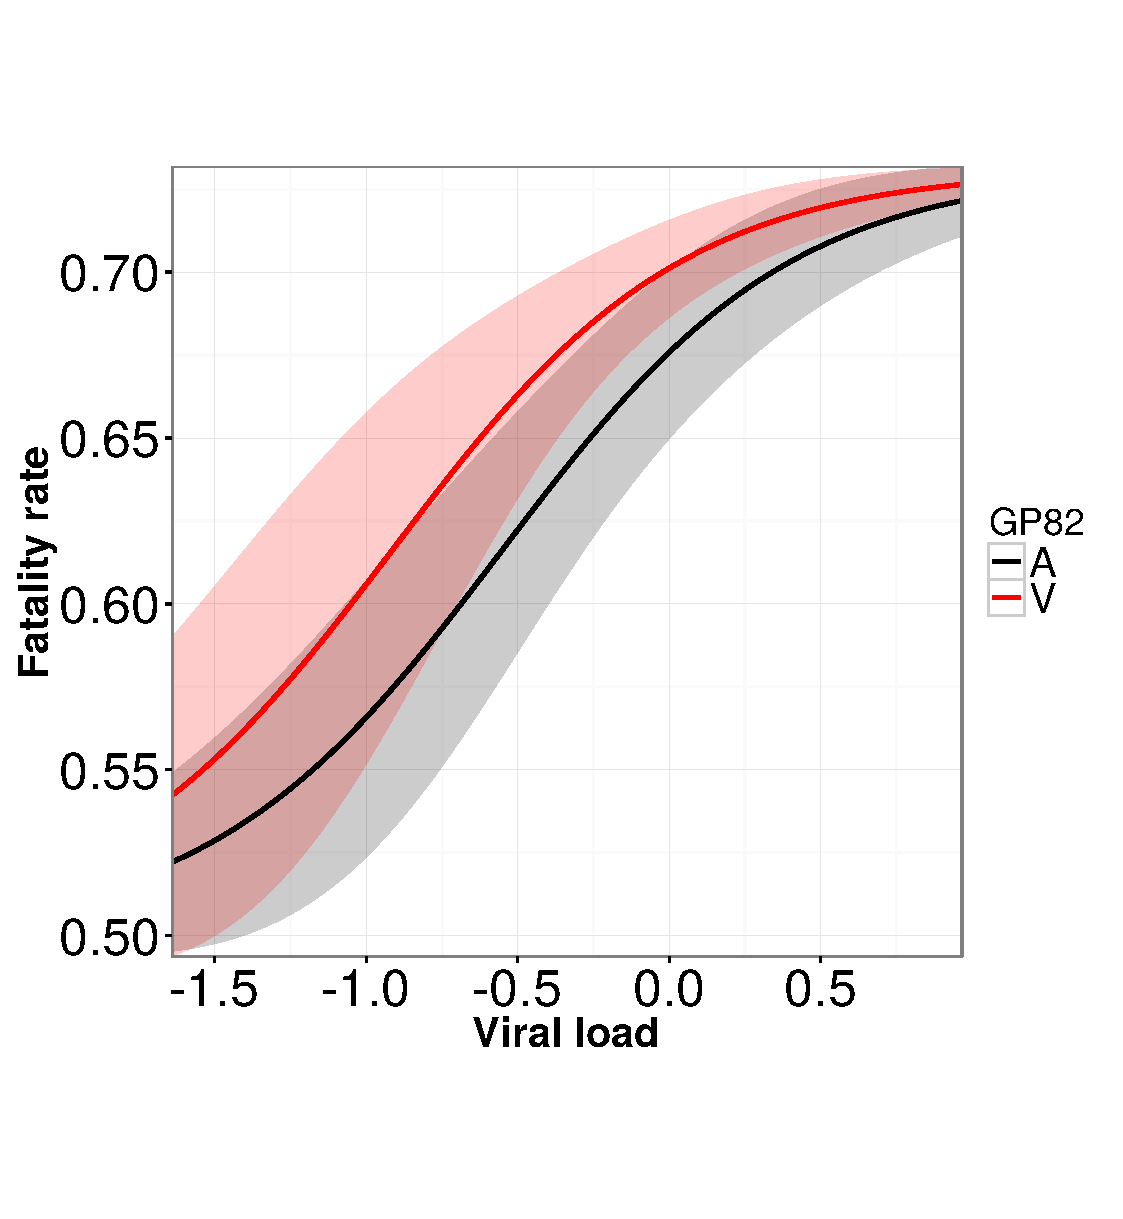
\includegraphics[scale=0.35,valign=c]{images/predicted_fatality_rates.pdf}
\end{tabular}
\textbf{Answer:} Yes, there is some evidence that A$\rightarrow$V conferred increased infectivity intra-host.
That does not mean the mutation had any bearing in transmission, however.
\section*{ What drove the epidemic?}
%  \begin{tabular}{cc}
%  \includegraphics[scale=0.18,valign=c]{images/case-count_coefficients_crp.png} &
%   \includegraphics[scale=0.7,valign=c]{images/case-count_coefficients.png} 
%  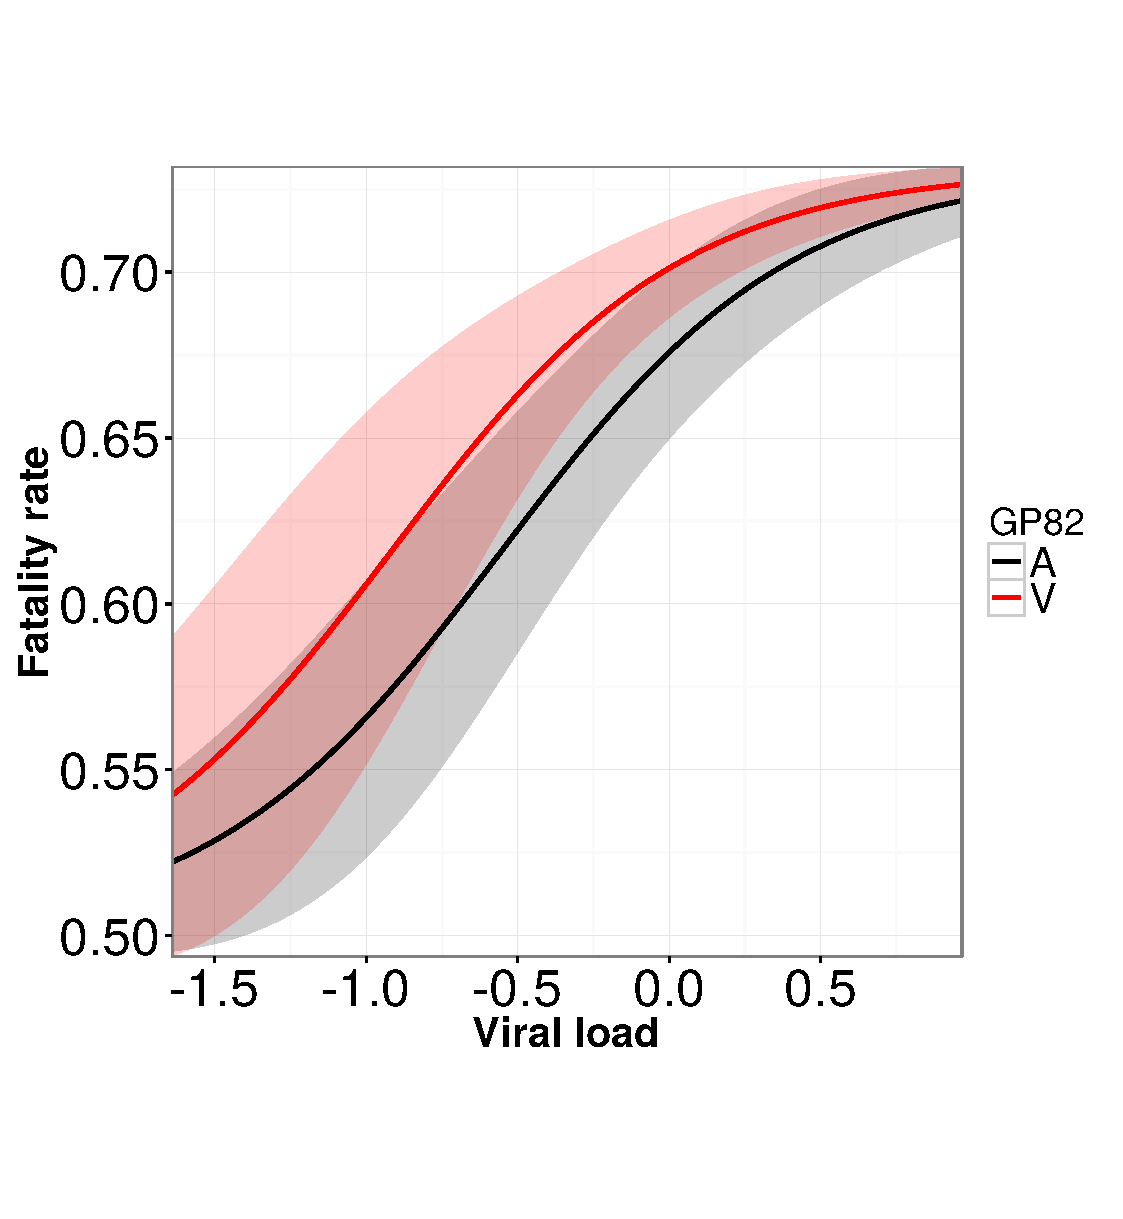
\includegraphics[scale=0.35,valign=c]{images/predicted_fatality_rates.pdf}
% \end{tabular}
\includegraphics[scale=0.18,valign=c]{images/case-count_coefficients.png}\\
%   \includegraphics[scale=0.75,valign=c]{images/case-count_coefficients.png} \\
\section*{Combining epidemiological and phylodynamic data}
 \begin{tabular}{ccc}
 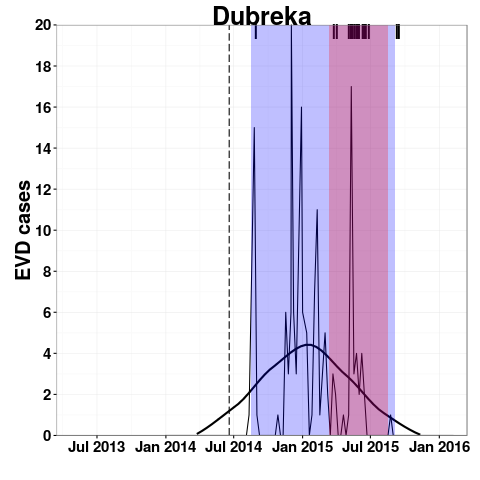
\includegraphics[scale=0.265]{images/maxCases_Dubreka.png} &
           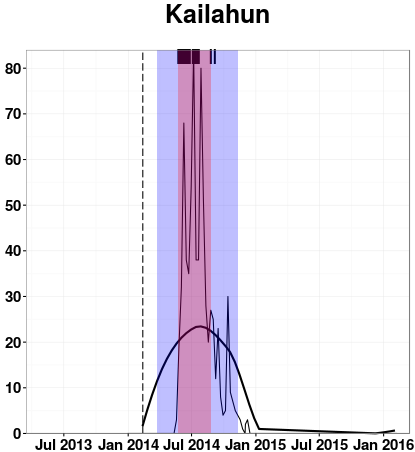
\includegraphics[scale=0.265]{images/maxCases_Kailahun.png}&
           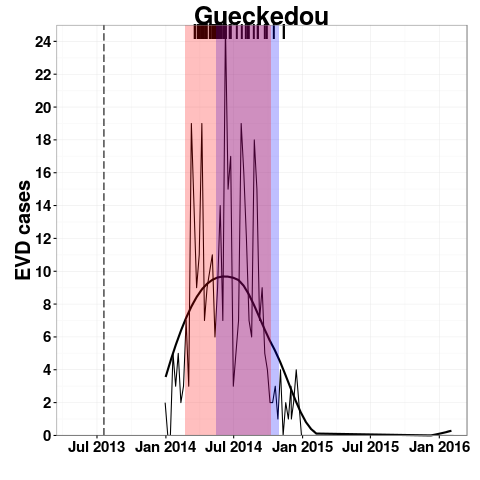
\includegraphics[scale=0.265]{images/maxCases_Gueckedou.png}
\end{tabular}
}
%%%%%%%%%%%%%%%%%%%%%%%%%%%%%%%%%%%%%%%%%%%%%%%%%%%%%%%%%%%%%%%%%%%%%%%%%%%%%%
  \headerbox{Thanks for reading!}{name=source,column=2,below=results,above=bottom}{
%%%%%%%%%%%%%%%%%%%%%%%%%%%%%%%%%%%%%%%%%%%%%%%%%%%%%%%%%%%%%%%%%%%%%%%%%%%%%%
I'm very grateful to IEB and SBS for topping up my annual stipend.
Thanks!
% % % % 
Source code and a cool animation showing the spread of A82V in West Africa are available at~\url{https://github.com/maxbiostat/diehl_ebola_cell_2016}.
A digital copy of this poster can be found at~\url{https://github.com/maxbiostat/second_year_poster}.
}
%%%%%%%%%%%%%%%%%%%%%%%%%%%%%%%%%%%%%%%%%%%%%%%%%%%%%%%%%%%%%%%%%%%%%%%%%%%%%%
  \headerbox{What's next?}{name=questions,column=1,span=1,below=results,above=bottom}{
%%%%%%%%%%%%%%%%%%%%%%%%%%%%%%%%%%%%%%%%%%%%%%%%%%%%%%%%%%%%%%%%%%%%%%%%%%%%%%
\begin{itemize}
 \item[\blacktriangleright] What impact did intervention have? $\rightarrow$ hierarchical SIR model;
 \item[\blacktriangleright] Study the correlation between viral load and fatality using a latent liability model;
 \item[\blacktriangleright] Investigate possible differences in rates of evolution across time and space;
\end{itemize}
  }
%%%%%%%%%%%%%%%%%%%%%%%%%%%%%%%%%%%%%%%%%%%%%%%%%%%%%%%%%%%%%%%%%%%%%%%%%%%%%%
  \headerbox{Methods}{name=method,column=0,below=contribution,above=references}{
%%%%%%%%%%%%%%%%%%%%%%%%%%%%%%%%%%%%%%%%%%%%%%%%%%%%%%%%%%%%%%%%%%%%%%%%%%%%%%
In total $1610$ genomes were sequenced so far.
We take a Bayesian approach and estimate time-calibrated phylogenies with \textbf{BEAST}.
\begin{itemize}
 \item[$\oint$] We had viral load ($C(t)$ values) and outcome (death/survival) information for $236$ patients $\rightarrow$ binomial GLM;
 \item[$\oint$] Case counts ($\mathbf{Y}$) along climatic and socio-economic covariates ($\mathbf{X}$) for $56$ locations $\rightarrow$ negative binomial GLM + SSVS:
\begin{align*}
 Y_i & \sim \text{NegBin}(p_i, r) \\
 p_i & = \frac{r}{(r + \lambda_i)}  \\ 
\log(\lambda_i) &= \alpha + \beta_{1}\delta_{1} x_{i1} + \ldots + \beta_{P}\delta_{P} x_{iP} 
\end{align*}
% % % % % % % % % 
 \item[$\oint$] Constructing outbreak clusters: every time a location receives a viral introduction that leads to $>$20 sampled cases, split the series before and after the introduction.
\end{itemize}
}
\end{poster}
\end{document}